\documentclass{beamer}

\setbeamertemplate{navigation symbols}{}

\usepackage{graphicx}
\usepackage{amsmath, amssymb, amsfonts, amsthm}
\usepackage{tabularx}

\usetheme{CambridgeUS}


%-----------------------------------------------------------------------------------------------------------------
% New Environment for a plain box
\newenvironment{boxeded}
    {\begin{center}
    \begin{tabular}{|p{0.9\textwidth}|}
    \hline\\
    }
    { 
    \\\\\hline
    \end{tabular} 
    \end{center}
    }
%-----------------------------------------------------------------------------------------------------------------

% Die Präsentation dient dem Praxisprojekt: COVID-19 und wurde von Regina Galambos und Lorenz Mihatsch erstellt.

% Folgende Inhalte sollen besprochen werden: 
% 1: Datenstruktur und -erhebung erläutern:
% 1.1) Probleme der Erhebung: Recoding policy, testing policy.
% 2: Fallzahlen Weltweit als Timescale und als Weltkarte bezogen auf 100k Einwohner
% 3: Wachstumsraten der Fallzahlen
% 4: Ländervergleich. Zentrieren um Tag der Abriegelung irgendeiner Art.






%-----------------------------------------------------------------------------------------------------------------
% Presentation information: title, author.....

\title[Praxisprojekt: COVID-19]{Analyse der COVID-19 Fallzahlen}
\subtitle{Praxisprojekt}
\author[R.Galambos, L.Mihatsch]{Regina Galambos, Lorenz Mihatsch\\
	
\includegraphics[width=0.22\textwidth]{LMU.pdf}\\
	{\small Projektpartner: Andr\'{e} Klima}}
%-----------------------------------------------------------------------------------------------------------------


%-----------------------------------------------------------------------------------------------------------------
% Begin of presentation.

%Title page
\begin{document}
\begin{frame}
	\titlepage
\end{frame}

% Table of contents
\begin{frame}
   \frametitle{Inhaltsangabe}
   \tableofcontents
 \end{frame}
 
 
 % Einführung
 %-----------------------------------------------------------------------------------------------------------------
 \section{Einführung}
 \begin{frame}
 	\frametitle{COVID-19 Pandemie}
	Kommentar: Pandemie erklären. Datenerhebung der John Hopkins Universität.
	Weg App erwähnen mit Interaktiven Graphiken und dem Link.
 \end{frame}
 \section{Daten}
  
 \begin{frame}
 	\frametitle{Daten}
	Erklärungen zum Datensatz und Abruf der Daten über RamiKrispin
	Weitere Teildatensätze: Kontinente, Population und Länderfläche.
	Klar machen, dass es sich um Reported Cases handelt.
	Umgang mit Diamond Pincess und MS Zaandam erklären: Rauslassen.
 \end{frame}
 
 \section{Weltweit}
 \begin{frame}
 	\frametitle{Kumulative Daten weltweit}
	Kommentar: Cumulative Daten der Welt als Timeline. Graphik mit Cases, Death und Recovered.
	Aus Zeitlichen Gründen wird "Recovered" aus der Präsentation weggelassen.
	Plot der Kumulativen Fallzahlen ab 100 Fälle mit den Linien der Verdoppelungszeiten?
	
 \end{frame}
 
\section{Wachstumsfaktoren}
\begin{frame}
\frametitle{Wiederholung: Wachstumsfaktor und geometrisches Mittel}
	\begin{boxeded}
	\textbf{Definition 1} \textit{Wachstumsfaktor}\\
	Sei $C_0, C_1, C_2, ...$ eine Zeitreihe von Fallzahlen zu den Zeitpunkten $0, 1, ..., n$. Dann ist für $i = 1, ..., n$ der i-te Wachstumsfactor $x_1$ gegeben durch $$ x_i = \frac{C_i}{C_{i-1}}.$$
	\end{boxeded}

	Die Fallzahlen $C_n$ zum Zeitpunkt $n$ sind gegeben durch $$C_n = C_0 \cdot x_1 \cdot x_2 \cdot ... \cdot x_n$$
\end{frame}

\begin{frame}
\frametitle{Wiederholung: Wachstumsfaktor und geometrisches Mittel}
	\begin{boxeded}
	\textbf{Definition 2} \textit{Geometrisches Mittel}\\
	Das geometrische Mittel zu den Wachstumsfaktoren $x_1, x_2, ..., x_n$ ist gegeben durch $$\bar{x}_{geom} = (x_1 \cdot x_2 \cdot ... \cdot x_n)^{1/n}.$$ Daraus ergibt sich $C_n = C_0 \cdot x_1 \cdot x_2 \cdot ... \cdot x_n = C_0 \cdot (\bar{x}_{geom})^n$.
	\end{boxeded}
	\pause
	Wir betrachten im Folgenden den \emph{rolling geometric mean} der vergangenen 7 Tage. Dazu berechnen wir für jeden Zeitpunkt $i$ $$\bar{x}_{i, geom} = (x_i \cdot x_{i-1} \cdot x_{i-2} \cdot ... \cdot x_{i-6})^{1/7}.$$


\end{frame}

\begin{frame}
\frametitle{Wachstumsfaktoren}
	\begin{figure}
		\centering
		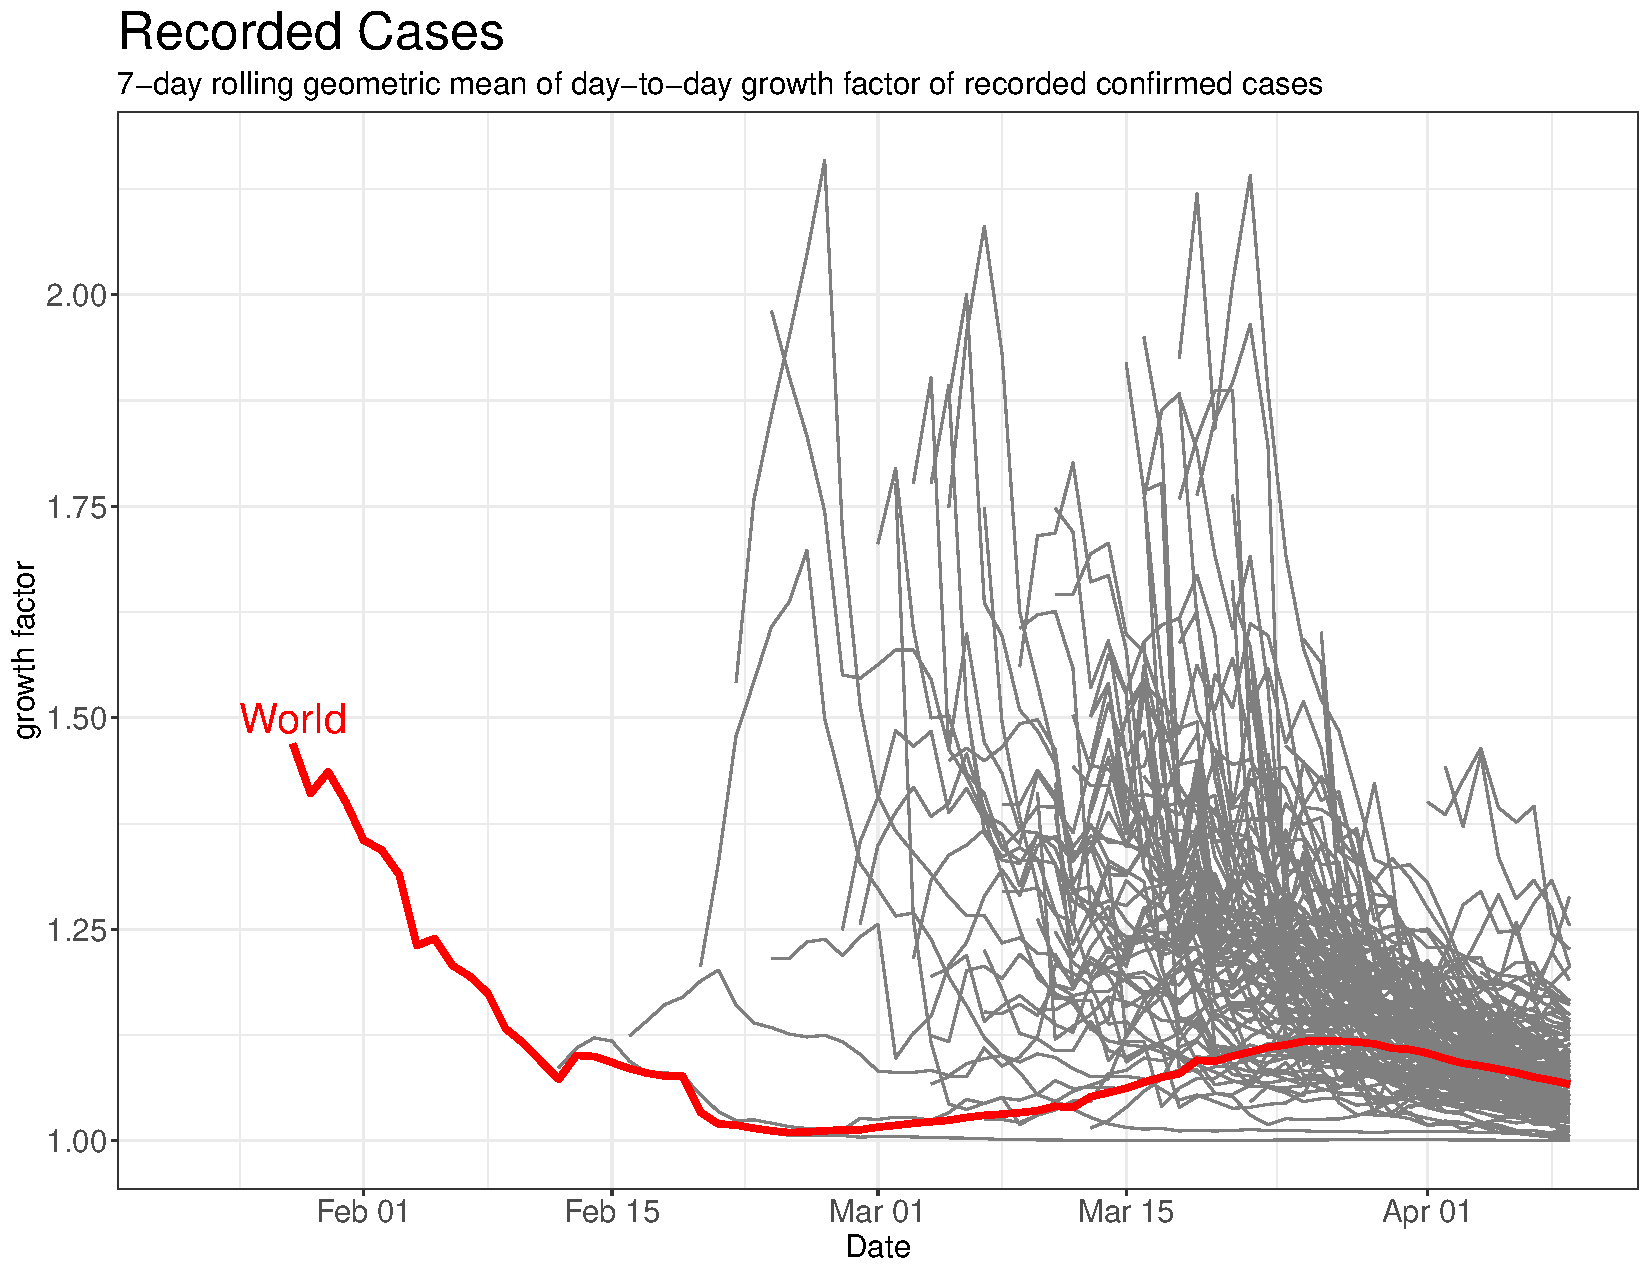
\includegraphics[width = 270pt]{GF_confirmed}
	\end{figure}
\end{frame}

\begin{frame}
\frametitle{Wachstumsfaktoren}
	\begin{figure}
		\centering
		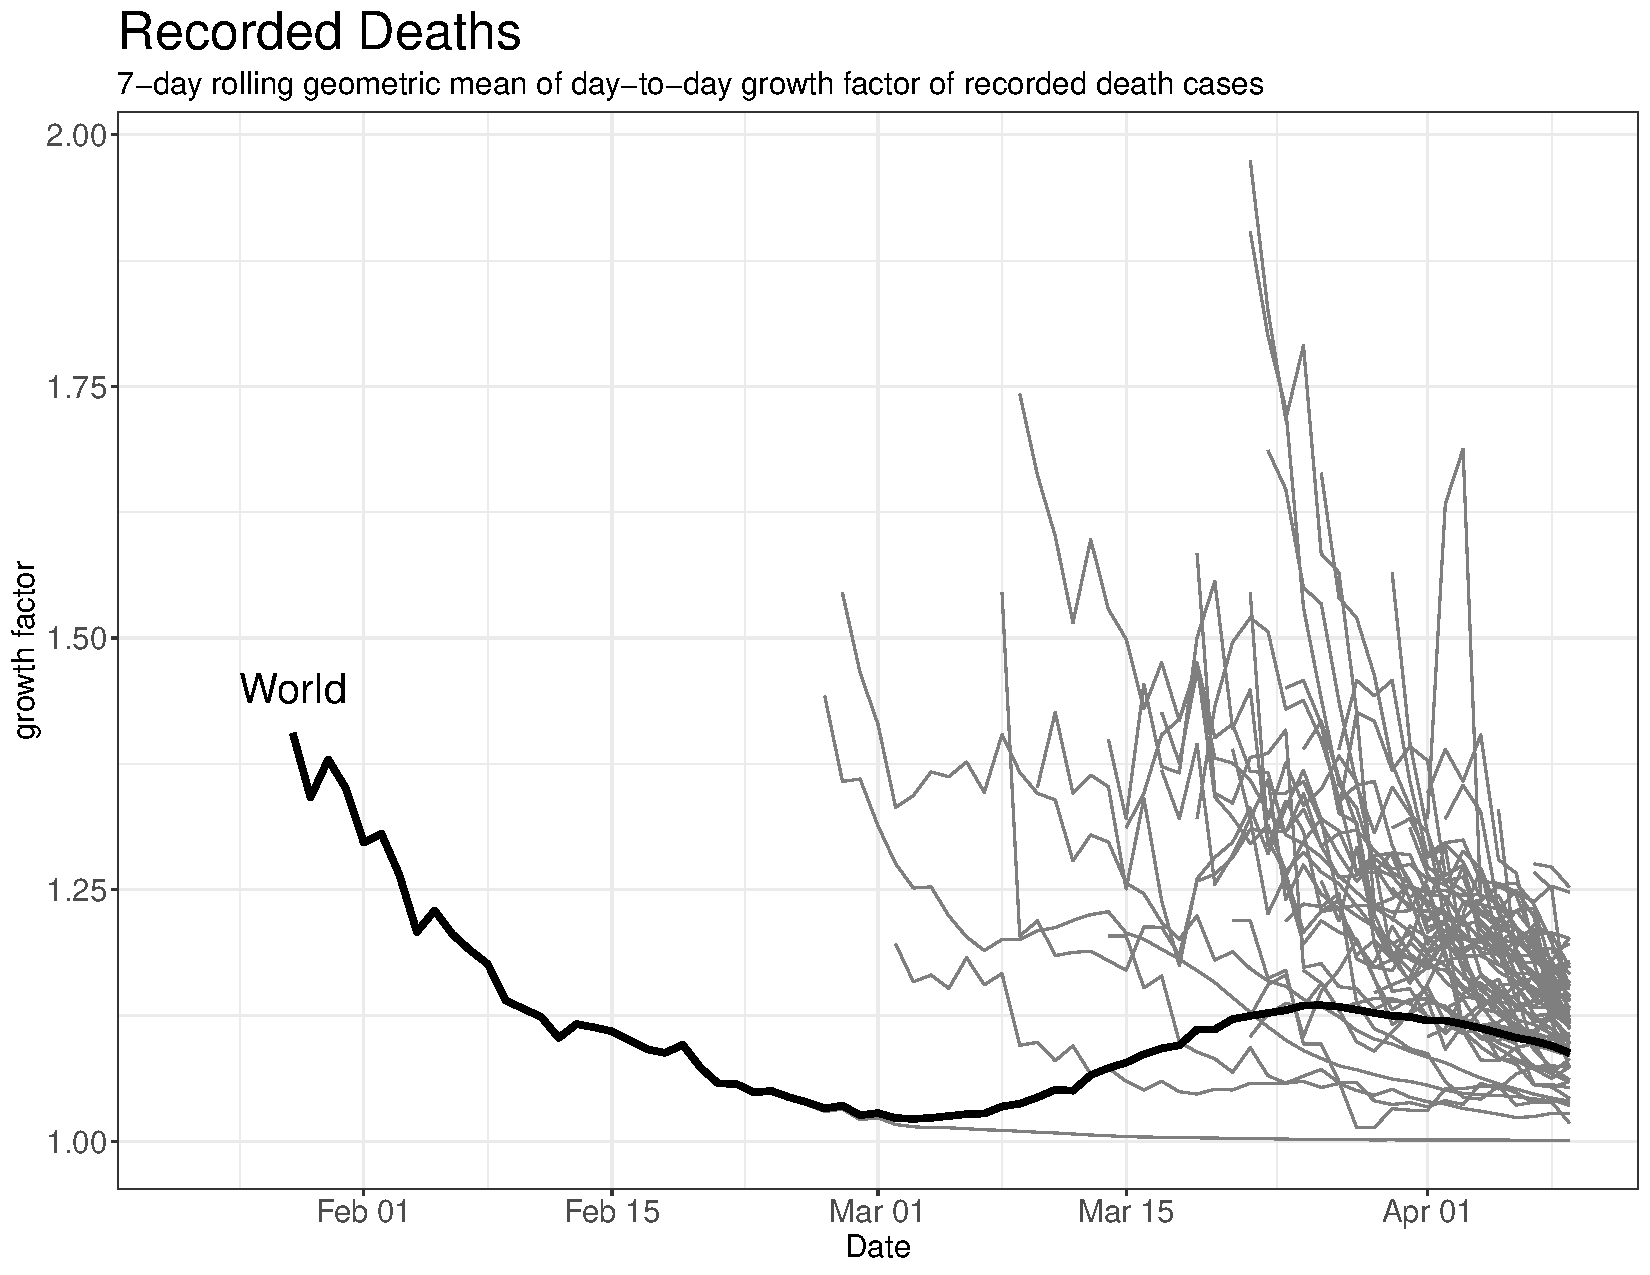
\includegraphics[width = 270pt]{GF_deaths}
	\end{figure}
\end{frame}

\begin{frame}
\frametitle{Verdopplungszeit}
	Ausgehend von einem exponentielle Wachstum der Form $C_n = C_0 \cdot (\bar{x}_{n, geom})^{n}$ ergibt sie die "momentane" Verdopplunszeit $dt_i$ der Fallzahlen durch $$dt_i = \frac{ln(2)}{ln(\bar{x}_{i, geom})}.$$
	\pause
	\emph{Herleitung}: 
	\begin{align*} C_i \cdot (\bar{x}_{i, geom})^{dt_i} = 2 \cdot C_i 
	 &\iff (\bar{x}_{i, geom})^{dt_i} = 2 \\
	 &\iff dt_i = \frac{ln(2)}{ln(\bar{x}_{i, geom})}.
	\end{align*}
\end{frame}

\begin{frame}
\frametitle{Verdopplungszeit: Bestätigte Fälle}
	\begin{figure}
		\centering
		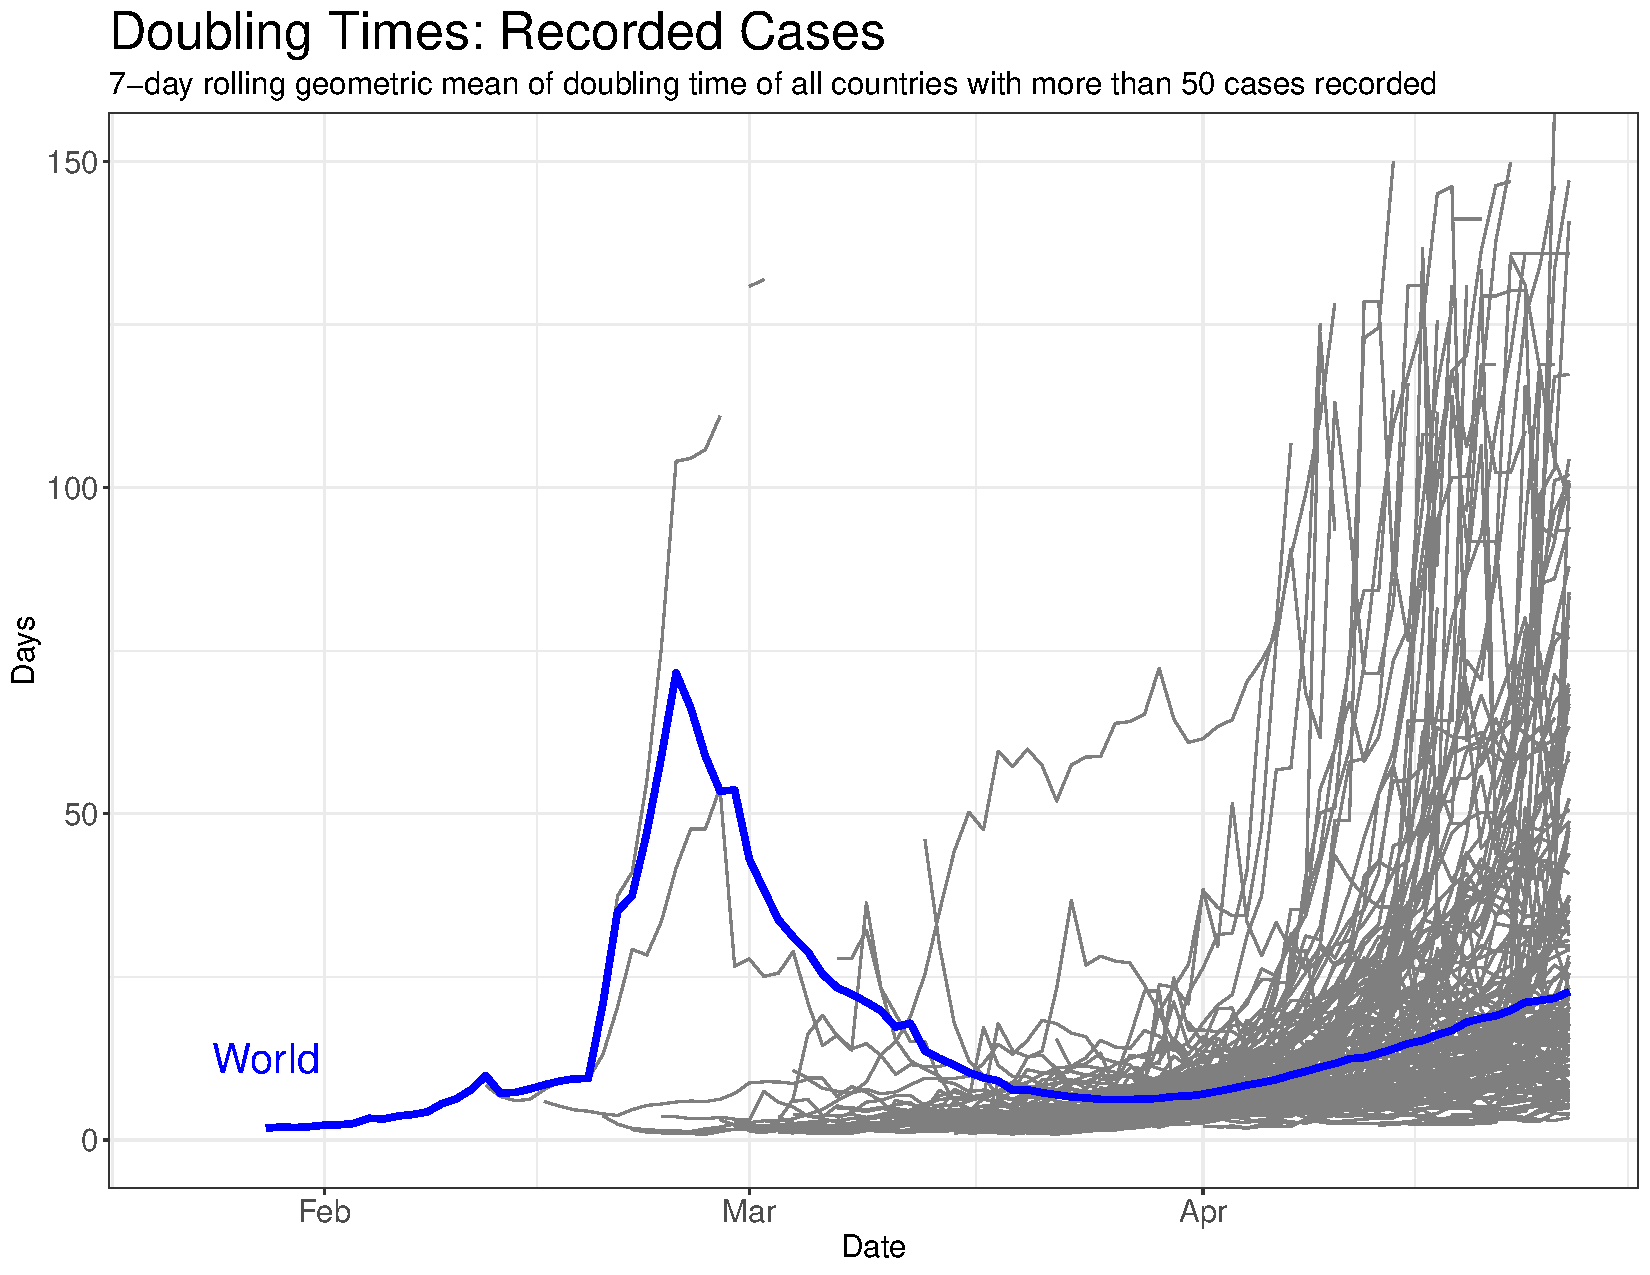
\includegraphics[width = 270pt]{DT_confirmed}
	\end{figure}
\end{frame}

\begin{frame}
\frametitle{Verdopplungszeit: Todesfälle}
	\begin{figure}
		\centering
		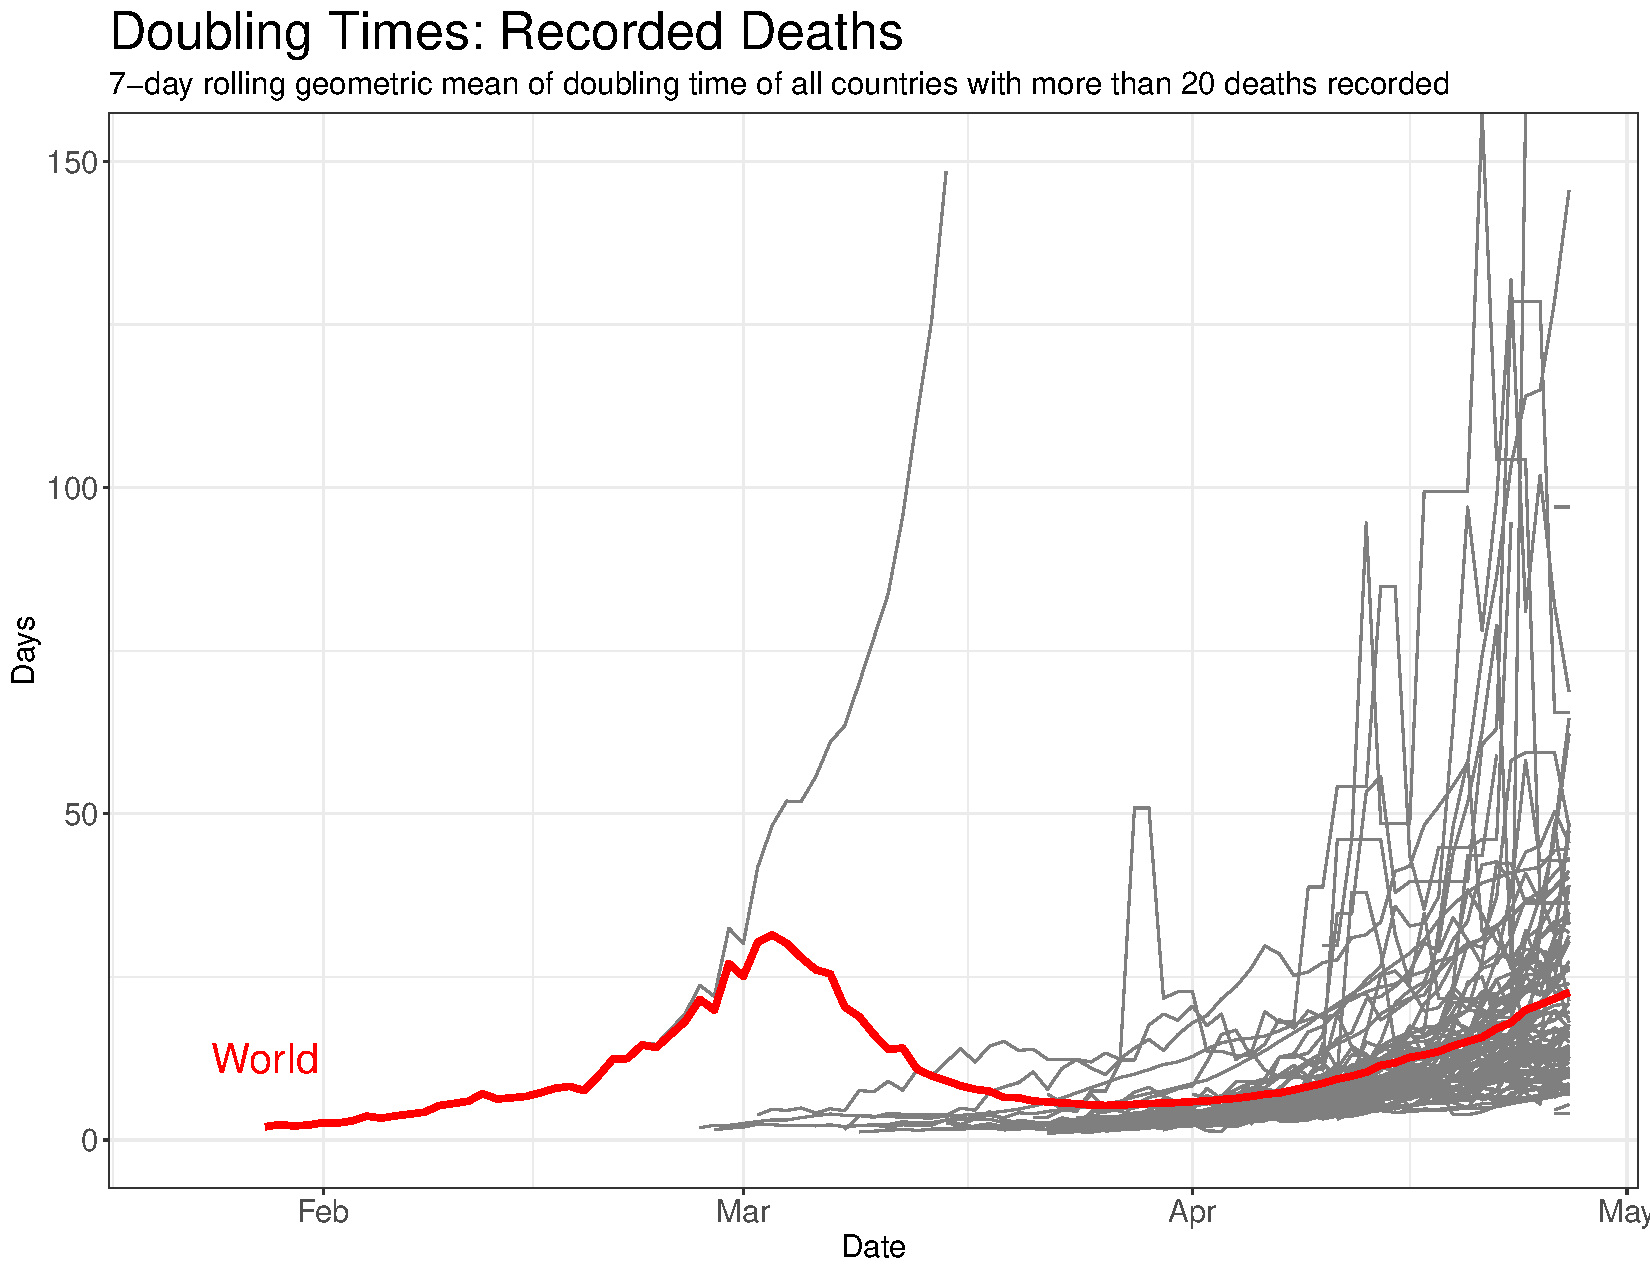
\includegraphics[width = 270pt]{DT_deaths}
	\end{figure}
\end{frame}

 \section{Ländervergleich}
\begin{frame}
\frametitle{Infektionsmaßnahmen}
	Kommentar: Beispiel Plot von South Korea um Problematik der Zentrierung zu erläutern. Wachstumsraten bzw. Verdoppelungszeit zentriert um die Einführung der Maßnahmen.
\end{frame}

\begin{frame}
\frametitle{Diskussion}
	\begin{itemize}
		\item Die Berechnung des \emph{geometrischen Mittels der Wachstumsfaktoren} und der \emph{Verdopplungzeit} beruht auf der Annahme eines exponentielle Wachstums. Zulässigkeit?
		\item Weitere
	\end{itemize}
\end{frame}
 
\end{document}